% Sample Paper for Poster Conference
%( without guarantee:-)) 
%send your comment to xrund@fel.cvut.cz
%
\documentclass{poster16}
% 
%----------------------------------------------------------
%             THIS IS THE PLACE FOR YOUR FAVORITE PACKAGES
%
%\usepackage[latin2]{inputenc}%
%\usepackage{babel}% 
%\usepackage{czech}%
%\usepackage{psfrag}
%\usepackage{amsmath}
%\usepackage{pifont,amssymb}

\begin{document}
%----------------------------------------------------------

%----------------------------------------------------------
%               THIS IS THE PLACE OF THE TITLE
%
\title{Magnetometer Based Wind Vane}
%----------------------------------------------------------
%               THIS IS THE PLACE FOR THE AUTHORS NAMES AND THE TITLE FOR HEADINGS
%
\headtitle{F. S. AUTHOR, S. S. AUTHOR, SAMPLE PAPER FOR POSTER 2016 CONFERENCE}
%----------------------------------------------------------
%               THIS IS THE PLACE FOR THE AUTHORS NAMES - ALL AUTHORS MUST HAVE A STUDENT STATUS!!!

%
\author{Jakub Kakona \affiliationmark{1}}
%----------------------------------------------------------
%              THIS IS THE PLACE FOR AFFILIATIONS
%
\affiliation{%
\affiliationmark{1}Dept. of Radio engineering, Czech Technical University, Technick\'a 2, 166 27 Praha, Czech Republic}
  \email{kakonjak@fel.cvut.cz}
%--------------------------------------------------------------


\maketitle

%----------------------------------------------------------
%               THIS IS THE PLACE FOR ABSTRACT

\begin{abstract}
Wind vane sensor is classical meteorology instrument used for measuring wind directions. Wind directions are reported relatively to the magnetic north of weather station coordinates. Therefore precise directional adjustment of the sensor is needed. We introduced a self calibrating wind vane sensor which report the wind direction data without adjustments. Therefore it is more tolerant to the installation mistakes. 
\end{abstract}

%----------------------------------------------------------
%               THIS IS THE PLACE FOR KEYWORDS
\begin{keywords}
Wind sensor, 3D printing, scientific instrumentation.
\end{keywords}

%----------------------------------------------------------
%               HERE WRITE YOUR PAPER

\section{Introduction}

Wind vane is classical measuring device in meteorology. It is used for wind direction sensing at automatic weather stations. The classical construction of such sensor consist a analogue resistive position sensing or "digital" magnetic leaf switch contacts. Both discrete and continuous signal sensing approach measure the position of wind vane relatively to the local word coordinates. Although the wind direction is reported relatively to the magnetic north of weather station location. Therefore the precise direction adjustment of wind vane sensor is mandatory for achieving consistent and reliable wind direction data.

But we could use the state of the art technology consisting of MEMS magnetometer sensors which could directly report the wind vane position relatively to the magnetic north. This concept of wind vane is unique because it report continuous values which allows reliable auto-diagnostics of sensing element. 

\section{Design evolution}

The construction of the wind vane should be special because the sensing element in rotor part. The sensor is MAG01A module from MLAB electronic development system. This sensor is a I2C bus based sensor which requests four signals - Power, Ground, Data and clock. 

Therefore the one of main design problem is signal conduction from rotary part to the stator. A commercially available slip-rings were used as solution for that. 
The used slip-ring is shown in the figure X. 


The integration of such device in to the wind vane construction needs special shape of the rotor and the stator part. A 3D printing technology is ideal for that task. We decided to use the Fused deposition modelling (FDM) additive manufacturing technology as a best candidate for anemometer sensor design. The main reason for that decision was a fact, that this type of 3D printing technology is widely accessible and is of sufficient quality to build the sensor body which could withstand the mechanical and weather stresses in outdoor. The second reason is the fact that this type of technology is relatively  cheap in comparison to other additive manufacturing methods. 
But there also exist technological limits due to the fact that not all shapes could be 3Dprinted. The problematic geometry include overhanging surfaces or large number of very small details in printed volume. 

The design of wind vane therefore must have special construction which allows reliable printing without costly model specific G-code tweaking. Which is common practice to print poorly designed model on lower quality printers. 

\begin{figure}[ht]
\begin{center}
\resizebox{\linewidth}{!}{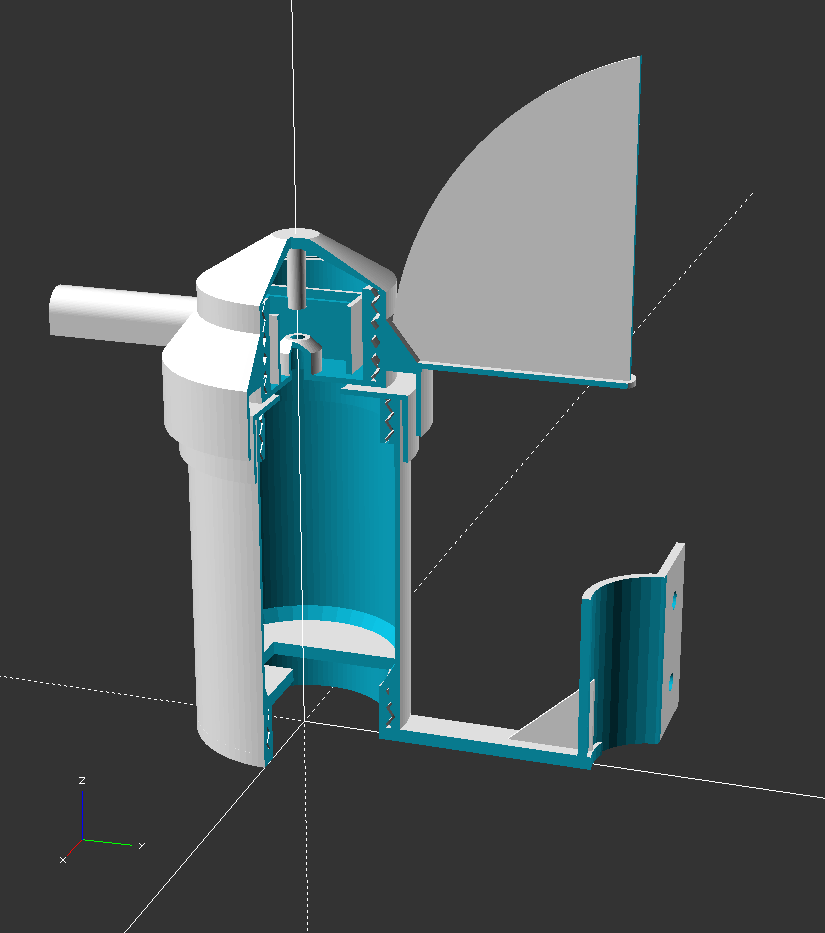
\includegraphics{./img/WINDGAUGE01A_Assembly.png}}
\caption{A sample of printable rocket design. (Experimentally printed from red ABS)} 
\label{fig:printed_parts}
\end{center}
\end{figure}


\subsection{Wind vane rotor}

The rotor part of the wind vane houses the magnetometer sensor. The MAG01A sensor module is triple axis one chip solution for magnetic orientation measurement. Sensor module is mounted directly in rotation center of wind wane, this position was choosed as the best option to optimizing the overall sensor dimensions. 

\subsection{Stator and holder}




\subsection{Software data processing}

The triple axis magnetometer sensor is read directly by pymlab sensor library, this library is primarily focused on I²C based sensor data reading.
Output of the magnetometer hardware driver is a uncalibrated vector of magnetic field.  Therefore a data calibration is needed to obtain a wind direction data. 



\section{Conclusion}

A considerable amount of development work resulted in a partially usable 3D printable rocket model. The FDM technology was proven to be a right selection. But large amount of development work will be needed to finish the rocket design to the level which will allow an easy usage by students. 
Specifically the following problems must be resolved before widespread usage: 

\begin{itemize}
\item Reliable recovery system
\item Easily producible rocket engine design  
\item On board avionics which could universally provide power source, recovery and measurement functions for any student payload. 
\end{itemize}

\section*{Acknowledgements}

The research presented in this proposal was not supported from any grant or from public resources. It was funded exclusively by Universal Scientific Technologies s.r.o. company. 

%----------------------------------------------------------
%               THIS IS THE PLACE FOR REFERENCES
\begin{thebibliography}{9}
\bibitem{rocket_sounding}
NASA Sounding Rockets User Handbook, Sounding Rockets Program Office,Sub-orbital and Special Orbital Projects Directorate
NASA Goddard Space Flight Center,Wallops Flight Facility, 23.3.2016 [online] http://sites.wff.nasa.gov/code810/files/SRHB.pdf
\bibitem{grid_fins}
Zaloga, Steve (2000). The Scud and Other Russian Ballistic Missile Vehicles. New Territories, Hong Kong: Concord Publications Co. ISBN 962-361-675-9.
\bibitem{openscad}
Marius Kintel et al.  23.3.2016 [Online]
http://www.openscad.org/about.html
\end{thebibliography}


%----------------------------------------------------------
%               THIS IS THE PLACE FOR AUTHOR CV
\begin{authorcv}{Jakub Kakona}
He is a Ph.D. student of  Air Traffic Control programme under Electrical Engineering and Information Technology. His professional activities are radioastronomy, development of 3D printers and scientific instruments design. 
\end{authorcv}
\end{document}

